\chapter*{Introduction}

\label{chap:intro}
\addcontentsline{toc}{chapter}{\nameref{chap:intro}}

\fancyhead[LO]{\sffamily\bfseries Introduction} % Print the nearest section name on the left side of odd pages
\fancyhead[RE]{\sffamily\bfseries Introduction} % Print the current chapter name on the right side of even pages




In our quest to describe and understand the world with physics, our intuition tells us to start with the small and the simple before working our way up to larger scales and more complex problems. This is the path we follow when we are first taught about atomic physics and start with the smallest existing atom, Hydrogen. Even before we know about quantum mechanics, we are often taught how to use simple Newtonian mechanics to calculate the circular movement of the Hydrogen electron around the nucleus in the historical Rutherford model. If we now aim at describing a slightly more complex atom, let us say Carbon for instance, we need to consider the electrostatic forces exerted by the nucleus on each of the 6 electrons as well as between each of the electrons. We are then quickly overcome by a feeling of helplessness at the sight of the equations we would have to solve.


This kind of problem is obviously not restricted to the description of atoms and is actually found in many areas of physics. Would we want to study an ensemble of celestial objects orbiting around a star, electrons in a copper wire, molecules in a gas, atoms in a solid or even how a crowd behaves, a thorough description of these systems would require to account for the motions of all the individual bodies and the interactions between each one of them, leaving us with an enormous amount of degrees of freedom and equations to solve. This is even more so true as the number of particles gets very large in these problems: a good order of magnitude is the Avogadro number $\mathcal{N}_A = 6.02 \times 10^{23}$, giving the number of Carbon 12 atoms in only $12\rm{g}$ of Carbon! These problems are regrouped under the denomination ``\textbf{many-body} problems''. 


Actually, many-body problems are not entirely impossible to approach theoretically. To do so, we need to go against our intuition to decompose the system into its elementary components and rather see it as a whole to study some kind of \textbf{averaged} behavior. This idea is for instance at the core of the field of Thermodynamics which aims to describe macroscopic properties of large numbers of particles, such as its temperature, pressure, entropy etc. representing ensemble averages independent from the dynamics of the individual components of the system. Another famous approach that relies on averaging to study interacting many-body systems is the \textbf{mean-field approximation}. The idea is to approximate the action of every particle of the system on a single one as an averaged effect, reducing the many-body problem to an effective one body problem that me way be able to solve.

\section*{Quantum physics}

When we study many-body problems where the individual constituents are the (almost) smallest brick of matter, namely electrons and atoms, we enter the realm of \textbf{quantum mechanics}. The key concept to understand when a system requires a quantum treatment is the de Broglie wavelength. In 1923 \cite{debroglie:tel-00006807}, the french physicist Louis de Broglie took the hypothesis of M. Planck and A. Einstein that light could have a corpuscular aspect and turned it around by postulating that matter could behave as a wave with a wavelength $\lambda_{\rm{dB}}$ equal to:

\begin{equation}
    \lambda_{\rm{dB}} = \frac{h}{m\bm{v}}
\end{equation}

\noindent where $m\bm{v}$ is the momentum of the particle that also writes $\hbar \bm{k}$ in quantum mechanics. Strictly speaking, $\bm{k}$ designs a wave vector but we will identify it to the momentum in the rest of this manuscript. Translating this concept to many-body physics, when taking an ensemble of particles at temperature $T$, one can define the average De Broglie wavelength, also known as the thermal De Broglie wavelength as:

\begin{equation}
    \lambda_{\rm{dB}} = \frac{h}{\sqrt{2 \pi m \kB T}}
\end{equation}

\noindent If the typical inter-particle distance in the many-body ensemble is much larger than the thermal De Broglie wavelength, \ie $\lambda_{\rm{dB}}^3 n \ll 1$ with $n$ the density of particles, the wave character of the particles hardly plays a role as the different matter waves do not overlap and the system is properly described using classical physics. On the other hand, when $\lambda_{\rm{dB}}^3 n \sim 1$, the system shows quantum wave-like behavior. This regime is known as the \textbf{quantum degeneracy} regime. Importantly, this condition is most often met when considering the physics of electrons in condensed matter systems even at room temperature, due to their small mass $m_e = 9.1 \times 10^{-31} \ \rm{kg}$ and the high densities of electrons in solids of the order of $10^{29} \ \rm{m}^{-3}$.

The wave-like nature of the particles, as well as the effect of quantum statistics and quantum fluctuations observed in the quantum degeneracy regime brings out a large variety of fascinating and ``intuition-defying'' phenomena of which many are still not understood to this day, especially in many-body systems. For these reasons, quantum physics constitutes an exciting and leading area of modern day physics.

\section*{Interactions in quantum systems}

While approximate methods like the mean-field approach have been used with great success in the past to study quantum many-body problems, they nevertheless fail to characterize more strongly interacting systems for which beyond mean-field approaches are required \cite{navon2010equation,lavoine2021,papp2008bragg}. To properly describe these systems, it is then necessary to consider the dynamics of the individual components of the system \cite{hodgman2017solving,schweigler2017experimental,wenz2013few}. As a result, the modern day term ``many-body physics" usually refers to beyond mean-field approaches that account for the presence of \textbf{correlations} between the individual components of the system. Importantly, these correlation patterns get increasingly complex and contain more information as the interactions are strong. Consequently, a large part of quantum many-body physics is dedicated to studying how correlations emerge from the interplay between the inter-particle interactions and the quantum fluctuations and what they tell us of the physics of the system. This field of physics remains to this day a largely open field with a lot of unresolved questions concerning systems ranging from solid state physics to neutron stars, but that already found some great successes. We can mention the notable example of low temperature superconductivity studied by Bardeen-Cooper-Schrieffer \cite{bardeen1957theory} (BCS) in 1957 that described the superconducting current as a superfluid of Cooper pairs \cite{cooper1956bound}, where a Cooper pair is a pair of electrons bound by an effective attractive interaction (in this case the exchange of phonons). The existence of high temperature superconductors remains however unexplained to this day and constitutes a particularly interesting question of many-body physics.

\section*{Cold atoms and quantum simulation}

Even though we have understood that exact analytical approaches are almost always impossible to pursue in the case of quantum many-body systems, we could however think of using numerical techniques and the calculation power of modern-day super computers. Nevertheless, if we wish to consider all kinds of correlations between the particles, the size of the associated Hilbert space grows exponentially with the number of particles. This exponential growth considerably limits the number of particles that can be simulated, roughly to a hundred with modern day computers. In a famous paper of 1982 \cite{Feynman1982Simulating}, R. Feynman introduced the concept of \textbf{quantum simulation} by suggesting that quantum phenomena could be simulated using actual quantum components instead of classical computers. The idea is to simulate a system or an Hamiltonian of interest with a quantum platform on which one can (\textit{i}) precisely control all the relevant parameters and (\textit{ii}) measure the observables of interest. The technological developments of the past decades have made Feynman's idea come to life with increasingly more precise and efficient simulators implemented on a variety of platforms such as ions, superconducting qbits or ultracold gases. We will focus in this manuscript on this latter example.  

Contrary to condensed matter systems, ultracold gases are a dilute state of matter in the sense that they typically contain $10^5-10^7$ atoms in large volumes, resulting in much lower densities than those found in solids. As a result, at room temperature, these gases are far from being quantum degenerate. To reach the regime of quantum degeneracy, the gas must be cooled down to very low temperatures $\sim \mu \rm{K}$ to increase $\lambda_{\rm{dB}}$ until $\lambda_{\rm{dB}}^3 n$ reaches unity. When the atoms are indistinguishable  bosons, under a critical temperature associated with $\lambda_{\rm{dB}}^3 n \sim 1$, a macroscopic number of atoms occupy the lowest energy state of the system, forming a new state of matter called the \textbf{Bose-Einstein Condensate (BEC)}. Importantly, all the condensed atoms then form a single, \textbf{coherent} matter-wave. 

The field of ultracold atoms was born thanks to the discovery of laser cooling techniques \cite{chu1985three,dalibard1989laser,phillips1982laser} that allowed to reach such low temperatures and led to the observations of the first BECs by the teams of E. Cornell \cite{anderson1995observation} and W. Ketterle \cite{davis1995bose} in 1995. From this day, ultracold atoms and Bose-Einstein Condensates have been the subject of many experiments and brought a large variety of important results and several Nobel prizes.

Ultracold atoms are actually perfectly suited to study condensed matter as it is relatively easy to create all sorts of potentials to trap the atoms using laser light, with the notable example of optical lattices \cite{bloch2005ultracold} that reproduces the crystalline structure of solids. Another interesting properties of ultracold atoms is that the strength of the interactions of some atomic species\footnote{This is however not the case for metastable Helium-4 that we will study in this manuscript} can be tuned using Feshbach resonance \cite{chin2010feshbach,feshbach1958unified}. One may thus have a system in which one controls the number of particles, the properties of the crystal-like potential such as its geometry and the distance between the sites and finally the strength of interactions. Such quantum gas platforms fulfill the first condition for them to be an adequate quantum simulator of famous condensed matter models such as the Fermi- and Bose-Hubbard models for fermions and bosons respectively, or the Ising model. This level of control on the parameters of the simulated Hamiltonian would of course be useless if it were impossible to measure the properties of the system. One other significant asset of ultracold atoms in optical lattices systems is that they are actually relatively easy to probe.

\section*{Probing the momentum degree of freedom}

Recent optical lattices experiments can be categorized according to the kind of probes they use to study the many-body problem. A first technique consists in probing the excitations of the system, \ie how the system respond when extra energy or momentum is deposited in the system, to obtain information about the many-body states. This probe was developed in analogy to condensed matter approaches such as angle-resolved photoemission spectroscopy \cite{damascelli2003angle} or neutron scattering \cite{ashcroft1976solid}. For ultracold atoms systems, the excitations of the system can be probed using radio-frequency (RF) spectroscopy \cite{stewart2008using}, Raman spectroscopy \cite{dao2007measuring}, amplitude modulations of a 2D lattice revealing Higgs mode excitations \cite{endres2012higgs} or Bragg spectroscopy \cite{sobirey2021observation,steinhauer2002excitation}. Finally, the properties of the excitations can also be accessed by studying the out-of-equilibrium properties of the system \cite{keesling2019quantum,villa2019unraveling}.

Ultracold atoms platforms have brought up new ways to probe many-body systems differently from the techniques used in condensed matter experiments. It is notably possible to probe the position or spin degree of freedom using quantum gases microscopes \cite{bakr2009quantum,cheuk2015quantum,esteve2008squeezing,sherson2010single} capable of detecting the fluorescence of individual atoms trapped in the different sites of an optical lattice. These techniques allow to characterize many-body systems through the study of position and spin correlations between individual particles.

Finally, the same idea can be extended to the momentum degree of freedom. The momentum-space can be accessed through Time-Of-Flight (TOF) techniques \cite{greiner2002quantum,spielman2008condensate,xu2006observation} that consist in measuring the positions of the atoms after a time $t_{\rm{TOF}}$ of free expansion. In a very simple picture with classical particles that do not interact during the TOF, this position gives information about the in-trap momentum of the particle through the simple \textbf{ballistic relation}:

\begin{equation}
    \hbar \bm{k} = \frac{m \bm{r}}{t_{\rm{TOF}}}
\end{equation} 

The situation is actually more complex when accounting for the wave nature of the particles, as we will discuss later, but we can keep for now this simple picture. The combination of a TOF and a single-atom resolved detection technique allows to study momentum-space correlations between individual particles from which meaningful information about many-body systems can be obtained. The experiment that we will describe in this manuscript belongs to this last category that will be our main point of focus.



% The concept of Time-Of-Flight measurements is actually quite simple. The idea is to abruptly turn off the trapping potential to let the atoms expand freely and measure their positions $\bm{r}$ after a given TOF $t_{\rm{TOF}}$. In a very simple picture with classical particles that do not interact during the TOF, this position gives information about the in-trap momentum of the particle through the simple \textbf{ballistic relation}:

% \begin{equation}
%     \hbar \bm{k} = \frac{m \bm{r}}{t_{\rm{TOF}}}
% \end{equation}

% \noindent The situation is in reality more complex when accounting for the wave nature of the particles. This will be discussed in great details throughout this manuscript, but we can keep for now this simple image.

There are many motivations to measure the momentum distribution to study ultracold gases and many-body physics as a whole. One of the main advantages of the momentum distribution is to reveal the \textbf{coherence} properties of the system, that are themselves greatly influenced by the interactions and the induced correlations between the particles \cite{greiner2002quantum}. Indeed, the wave-function in momentum-space $\psi(\bm{k})$ is linked to the spatial wave-function $\phi(\bm{r})$ by the Fourier transform:

\begin{equation}
    \psi(\bm{k}) \propto \int {\rm d}\bm{r} e^{i \bm{k} \cdot \bm{r}} \phi(\bm{r})
\end{equation}

\noindent As the momentum density $\rho(\bm{k})$ writes $\rho(\bm{k})= |\psi(\bm{k})|^2$, we obtain \cite{pitaevskii2016bose}:

\begin{equation}
    \rho(\bm{k}) \propto \int {\rm d}\bm{R} e^{i \bm{k} \cdot \bm{R}} \int {\rm d}\bm{r} \phi^* (\bm{r}) \phi(\bm{r}+\bm{R}) \propto \text{FT} [g^{(1)} (\bm{R})]
\end{equation}

\noindent which tells us that the momentum distribution is obtained from the Fourier transform of the first order correlation function $g^{(1)}$ which contains information about the coherence properties of the system.
This is quite reminiscent of Optics in which far-field interference experiments are used to characterize the spatial and temporal coherence properties of a light source. With ultracold atoms, the light waves are replaced by matter-waves and the far-field regime of observation analog to the momentum distribution of the gas.

The momentum distribution was historically \cite{anderson1995observation} used to detect the presence of Bose-Einstein Condensation as illustrated on Fig.-\ref{fig:1st_BEC}. As the BEC is a fully coherent matter-wave, it manifests itself by the presence of sharp peak around zero momentum with a small width set by Heisenberg uncertainty principle as the atoms are spatially localized. The momentum distribution can also be used to study excitations, complementary to the methods cited earlier, signaled in momentum-space by the dispersion relation from which a variety of information can be obtained \cite{clement2009exploring,ozeri2005colloquium,sagi2012measurement}.


\begin{figure}
    \centering
    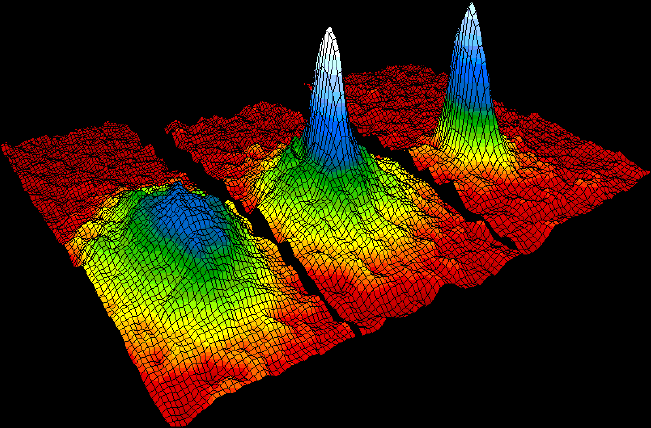
\includegraphics[width=0.7\textwidth]{Fig/Intro/BEC.png}
    \caption[Momentum distribution across Bose-Einstein Condensation]{Bose-Einstein Condensation. As temperature diminishes, the momentum distribution gets increasingly peaked around zero momentum. (JILA team, NIST USA)}
    \label{fig:1st_BEC}
\end{figure}


Last but not least, the momentum distribution also contains signatures of more complex interaction-induced correlation patterns between several individual particles. One of the most simple and famous example of such correlations are pairing mechanism inducing opposite momentum correlations. This is notably the case for two electrons belonging to a Cooper pair as discussed earlier, as well as for the \textbf{quantum depletion} of a BEC. The quantum depletion is the fraction of atoms removed from the condensate by the effect of inter-particle interactions and quantum fluctuations at zero temperature. It is an emblematic and conceptually simple example of a many-body effect. While the quantum depletion has already been observed \cite{chang2016,lopes2017,xu2006observation}, there have been no direct observation of pairing at opposite momentum expected for quantum depleted atoms. Obtaining this result will be the main point of focus of this manuscript.

\section*{Metastable Helium and electronic detection}

In order to detect such pairing correlations (or more complex correlation patterns with more than 2 particles that might be present in strongly interacting systems), a detection technique capable of resolving the momentum of each individual atoms of the gas is needed. Indeed, the idea behind correlation measurements is to measure the probability of \textbf{simultaneous} detection of several particles at specific momenta (for instance $\bm{k}$ and $-\bm{k}$). Many experimental efforts have been made in this direction in the past decades \cite{ott2016single}. While optical imaging techniques typically only allow to measure the \textbf{momentum density} of the gas rather than the full \textbf{momentum distribution}, some experiments such as the one led by S. Jochim in Heidelberg \cite{serwane2011deterministic} or by J. Schmiedmayer in Vienna \cite{bucker2009single} have adapted the quantum microscope technology to detect the fluorescence of single atoms after a TOF, thus obtaining a single-atom resolution in the momentum-space. However, the performances of these setups are somewhat limited by the properties of the imaging system, that requires the number of atoms to be kept relatively low so that the fluorescence patterns of the different atoms do not overlap for them to be resolved.

An alternative to optical probing is to use \textbf{electronic} detection techniques. In the early 2000s, the team lead by D. Boiron, C. Westbrook and A. Aspect at Institut d'Optique pioneered a new detection scheme exploiting the properties of the metastable state of the Helium atom that they managed to bring to quantum degeneracy in 2001 \cite{robert2001bose}. A great advantage of this method lies in its \textbf{3D} single-atom resolution as well as the possibility to implement it for systems with larger atom numbers of the order of $10^3-10^5$ (this must be nuanced by the fact that the detector saturates if the atomic flux is too high). In addition, this method allows to use large Times-Of-Flight to properly access the far-field regime of expansion in which the interferences are well resolved, in analogy to the Fraunhofer regime of diffraction\footnote{This point will be discussed in details in this manuscript}.

As we will see in this manuscript, a major drawback of this technique is that it only works with noble gases with a metastable state. To this day, Helium is the only noble gas that has been brought to quantum degeneracy (even though Neon, Argon and Krypton have been laser cooled \cite{katori1990laser,shimizu1989laser}), limiting the use of this detection technique to this single atomic species. To this day, there actually only a few metastable Helium experiments in the world: Canberra led by A. Truscott \cite{abbas2021rapid}, Vienna led by A. Zeilinger \cite{keller2014bose}, Amsterdam formerly led by W. Vassen \cite{mcnamara2006degenerate} with the fermionic isotope of Helium $^3 \rm{He}$ and two in Palaiseau, the historical one led by D. Boiron, C. Westbrook and A. Aspect and a second one led by D. Clément. This second metastable Helium experiment was built at Institut d'Optique starting in 2011, with the observation of Bose-Einstein condensation in 2015 \cite{bouton2015fast}. This new experiment implemented a new cooling sequence allowing to produce a BEC in $\sim 6\rm{s}$ instead of $\sim 30\rm{s}$ on the historical experiment, thus significantly speeding up the data acquisition time for the measurement of momentum correlations.

\section*{Optical lattices and the superfluid-to-Mott insulator transition}

The other specificity of this second experiment at Institut d'Optique is the use of optical lattices, from which the name of the team ``Helium Lattice'' derives. Optical lattices are particularly suited to study many-body, strongly interacting systems as the lattice potential locally increases the density and in turn the interactions, making phenomenon like quantum depletion even more pronounced than in regular harmonic traps. In addition, the Bose-Hubbard model predicts the existence of a phase transition from a superfluid phase to an insulating phase when the depth of the lattice potential increases known as the superfluid-to Mott insulator transition, first observed with cold atoms in 2002 \cite{greiner2002quantum} following the proposal of \cite{jaksch1998cold}. Studying momentum correlations all across the superfluid-to Mott insulator transition sets the general frame of the work presented in this manuscript, and conducted during my time as an intern and then as a PhD student in the Helium Lattice team that I had the chance to join in 2018.

\section*{Outline of the manuscript}

The manuscript is organized in five chapters. All chapters but the final one are centered around the common topic of the \kmk correlations in the quantum depletion of weakly-interacting lattice Bose gas.

\begin{itemize}
    \item The first chapter is dedicated to presenting the proper formalism to study quantum correlations. The concept of correlation functions is first introduced in the context of Quantum Optics and then extended to Atomic Physics. We then detail the main lines of the Bogoliubov theory of the homogeneous weakly-interacting Bose gas. We present what the quantum depletion is and where does the \kmk pairing comes from. Finally, we discuss some recent numerical calculations \cite{butera2020} of the correlations in the Bogoliubov theory for trapped systems, before presenting the essential experimental ingredients to observe the \kmk pairs.
    \item The second chapter is also a theoretical one and discusses the Bose-Hubbard model of bosons trapped in a 3D optical lattice. We explain what the superfluid-to-Mott insulator transition is and discuss the conditions under which the in-trap momentum distribution of the gas can be properly measured using a TOF technique, as well a the observability of the \kmk pairs of the quantum depletion in this system.
    \item The third chapter describes our experimental apparatus, namely the sequence used to produce a BEC of metastable Helium and the detection technique. In a second stage, we present two experimental measurements aimed at proving the points raised in Chapter \ref{sec:chapter_2}: one proving that we are able to adiabatically prepare an arbitrary state of the Bose-Hubbard model; a second one measuring beyond-mean field two-body collision effects happening during the TOF to prove that they are negligible in usual experimental conditions (therefore not detrimental to our measurement of the momentum distribution). 
    \item The fourth chapter details our experimental observation of the \kmk pairs of the quantum depletion. We describe the numerical procedure to analyze the data and study the characteristics of the experimental correlation signals in light of Bogoliubov theory: width, amplitude and dependency to temperature. We then perform complementary analysis of the data to obtain results leading towards probing the presence of entanglement in our system: we observe a relative number squeezing measurement between modes $\bm{k}$ and $-\bm{k}$, as well as a violation of the Cauchy-Schwarz inequality. Finally, we discuss some preliminary results on the evolution of the correlation signals with momentum $k$.
    \item The fifth and last chapter is separate from the rest of this manuscript and concerns a different project that was led during this thesis, the measurement of Tan's contact in 1D gases. We first introduce Tan's contact as well as the main results of a recent theoretical study \cite{yao2018tan} of the contact for trapped 1D bosons. We then present the procedure used to extract the contact from the raw experimental data and discuss the first preliminary results and their discrepancy with theory.
\end{itemize}









